\documentclass[aspectratio=169]{beamer}
\usepackage{lipsum}
\usefonttheme[onlymath]{serif} %Deja la misma fuente en el modo matemático igual que en artículo
%http://tex.stackexchange.com/questions/34265/how-to-get-beamer-math-to-look-like-article-math
%\usefonttheme{serif}
% There are many different themes available for Beamer. A comprehensive
% list with examples is given here:
% http://deic.uab.es/~iblanes/beamer_gallery/index_by_theme.html
% You can uncomment the themes below if you would l
%\usetheme{Montpellier}%$
%\usetheme{PaloAlto}%$
%\usetheme{Pittsburgh}%$
%\usetheme{Rochester}%$$ cuadros marcados rojo oscuro
%\usetheme{Singapore}%ike to use a different
% one: 
%\usetheme{AnnArbor}
%\usetheme{Antibes}
%\usetheme{Bergen}
%\usetheme{Berkeley}
%\usetheme{Berlin}
%\usetheme{Boadilla}
\usetheme{boxes}%$$rojo fuerte
%\usetheme{CambridgeUS}
%\usetheme{Copenhagen}
%\usetheme{Darmstadt}%$
%\usetheme{default}
%\usetheme{Frankfurt}%$
%\usetheme{Goettingen}
%\usetheme{Hannover}
%\usetheme{Ilmenau}
%\usetheme{JuanLesPins}
%\usetheme{Luebeck}
%\usetheme{Madrid}
%\usetheme{Malmoe}
%\usetheme{Marburg}
%\usetheme{Szeged}
%\usetheme{Warsaw}
\usepackage{graphicx}
\usepackage{caption}
\usepackage{subcaption}
\usepackage{media9} %Para poner videos
\usepackage{tikz}
\usetikzlibrary{arrows}
\usepackage{verbatim}
%Para hacer animaciones
\usepackage{animate}
\definecolor{UBCblue}{rgb}{0.5,0 , 0.13} % UBC Blue (primary)

\setbeamercolor{frametitle}{fg=UBCblue}
\setbeamercolor{title}{fg=UBCblue}
\setbeamercolor{mycolor}{fg=UBCblue}



%\usecolortheme{orchid}
\usecolortheme{beaver}

%Para tachar formulas
\usepackage{cancel}

\usepackage{multirow}
\usepackage[spanish]{babel}
\usepackage[utf8]{inputenc}
\usepackage{amsfonts}
\usepackage{amssymb}
\usepackage{amsthm}
\usepackage{mathrsfs}

\usepackage{graphicx}
\usepackage{enumerate}
\usepackage{hyperref}
\usepackage{multicol}


\usepackage{float}
\usepackage{caption}
\usepackage{subcaption}
\usepackage{booktabs}
\usepackage{multirow}
\usepackage{array}
\usepackage{wrapfig}
\newcommand{\PP}{\mathbb{P}}
\usepackage{color}
\usepackage{subfigure} 
\usepackage{pgfplots}

%graficos
\usepackage[top=3cm,left=3cm,right=3cm,bottom=3cm]{geometry}
% Scriptsize axis style.
\pgfplotsset{every axis/.append style={tick label style={/pgf/number format/fixed},font=\scriptsize,ylabel near ticks,xlabel near ticks,grid=major}}
\pgfplotsset{compat=newest}

\newtheorem{lem}{Lema}
\newtheorem{defi}{Definición}
\newtheorem{teo}{Teorema}
\newtheorem{prop}{Proposición}

\newcommand{\R}{\mathbb{R}}
\newcommand{\N}{\mathbb{N}}
\newcommand{\Z}{\mathbb{Z}}
\newcommand{\di}{\operatorname{div}}
\newcommand{\id}{\operatorname{Id}}
\newcommand{\diam}{\operatorname{diam}}
\newcommand{\rot}{\operatorname{rot}}
\newcommand{\interior}{\operatorname{int}}
\newcommand{\dd}{\operatorname{d}}
\def\V{\mathbb V}
\def\E{\mathcal E}
\def\X{\mathcal X}
\def\U{\mathbb U}
\def\B{\mathcal B}
\def\A{\mathbb A}
\def\V{\mathbb V}
\def\pb{\mathbb P}
\def\T{\mathbb T}
\def\C{\mathbb{C}}
\def\I{\mathcal I }
\def\M{\mathcal{M}}
\def\H{\mathcal {H}}




\newcommand{\verde}{\textcolor[cmyk]{1,0,1,0}}
\newcommand{\azul}{\textcolor{blue}}
\newcommand{\rojo}{\textcolor{red}}


%Para hacer valor absoluto y normas en tex
\providecommand{\abs}[1]{\lvert#1\rvert}
\providecommand{\norm}[1]{\lVert#1\rVert}

%Para poner displaystyle
\newcommand{\ds}{\displaystyle}

%Para hacer indicatrices

\usepackage{dsfont}

\newcommand{\indAA}[3]{\mathds{1}_{(#1,#2)}(#3)}
\newcommand{\indAC}[3]{\mathds{1}_{(#1,#2]}(#3)}
\newcommand{\indCA}[3]{\mathds{1}_{[#1,#2)}(#3)}
\newcommand{\indCC}[3]{\mathds{1}_{[#1,#2]}(#3)}
\newcommand{\ind}[1]{\mathds{1}_{#1}}

%Para poner en negrita modo matemático
\newcommand{\bs}{\boldsymbol}

%\title{Presentación MA6981}
%\title[Presentación ME6909-1]{\small{ME6909-1 Trabajo de título}{}
%\Large{Presentación de avance del 50\% \qquad \\ \qquad y Fenómenos de Concentración}}
\centering
\title[Presentación ME6909-1]{\Large{Convolutional RNN for RUL Prediction in Mechanical Systems}\qquad \\
\\
\qquad \small{Miembros de la comisión:}\\
\qquad \small{Enrique López Droguett, Viviana Meruane Naranjo, Patricio Loncomilla Zambrana}}


% A subtitle is optional and this may be deleted
\subtitle{}

\author[Nicolas Oyharçabal Astorga]{\Large{Nicolas Oyharçabal Astorga}}
% - Give the names in the same order as the appear in the paper.
% - Use the \inst{?} command only if the authors have different
%   affiliation.

\institute[DIMEC UChile] % (optional, but mostly needed)
%{\large{Departamento de Ingenier\'ia Matem\'atica\\
  %Universidad de Chile}}
% - Use the \inst command only if there are several affiliations.
% - Keep it simple, no one is interested in your street address.

\date{\today}
% - Either use conference name or its abbreviation.
% - Not really informative to the audience, more for people (including
%   yourself) who are reading the slides online

%\subject{Presentación Avance 50\%}[]
% This is only inserted into the PDF information catalog. Can be left
% out. 

% If you have a file called "university-logo-filename.xxx", where xxx
% is a graphic format that can be processed by latex or pdflatex,
% resp., then you can add a logo as follows:

% \pgfdeclareimage[height=0.5cm]{university-logo}{university-logo-filename}
% \logo{\pgfuseimage{university-logo}}

% Delete this, if you do not want the table of contents to pop up at
% the beginning of each subsection:


\setbeamertemplate{navigation symbols}{}

%Bloques
%\setbeamertemplate{blocks}[default]
%\setbeamertemplate{blocks}[rounded]
\setbeamertemplate{blocks}[rounded][shadow=true]



%Listas
\setbeamertemplate{items}[circle]
%\setbeamertemplate{items}[ball]
%\setbeamertemplate{items}[square]

%Ancho de los bloques
\addtobeamertemplate{block begin}{%
  \setlength{\textwidth}{1.0\textwidth}%
}{}

\addtobeamertemplate{block alerted begin}{%
  \setlength{\textwidth}{1.0\textwidth}%
}{}

\addtobeamertemplate{block example begin}{%
  \setlength{\textwidth}{1.0\textwidth}%
}{}

%hacer invisible
\setbeamercovered{transparent}

% Let's get started
\begin{document}


\begin{frame}[plain]{}


\includegraphics[height=0.35\textheight]{animate/fcfm.pdf}
%\begin{minipage}{1.6cm}
%			
\includegraphics[scale=.12]{escudoU2014.pdf}
%		\end{minipage}
%		\begin{minipage}[t]{12cm}
%			UNIVERSIDAD DE CHILE\\FACULTAD DE CIENCIAS FÍSICAS Y MATEMÁTICAS\\DEPARTAMENTO DE INGENIERÍA MECÁNICA
%\end{minipage}

    \maketitle
\end{frame}



\begin{frame}

\frametitle{Contenidos}
\tableofcontents
\end{frame}




\AtBeginSection
{
\begin{frame}{{Convolutional Recurrent Neural Networks For Remaining Useful Life Prediction in Mechanical Systems}}
\begin{center}
%{\Large Sección $\thesection$}
\begin{beamercolorbox}[
sep=8pt,center]{part title}
%\setbeamercolor{part title}{fg=UBCblue}
\usebeamerfont{part title}\usebeamercolor[fg=black]{part title}
\insertsection
\end{beamercolorbox}
\tableofcontents[currentsection,sectionstyle=hide,subsectionstyle=show/hide]
%\tableofcontents[currentsection,hideothersections]
\end{center}
\end{frame}
}

\section{Introducción}

\begin{frame}{Introducción}
\begin{block}{Motivación}
La predicción del la vida útil remanente de un sistema mecánico disminuye el riesgo a fallas catastróficas y los costos de mantención. Ejemplo:
\begin{figure}
  \centering
  \subfloat{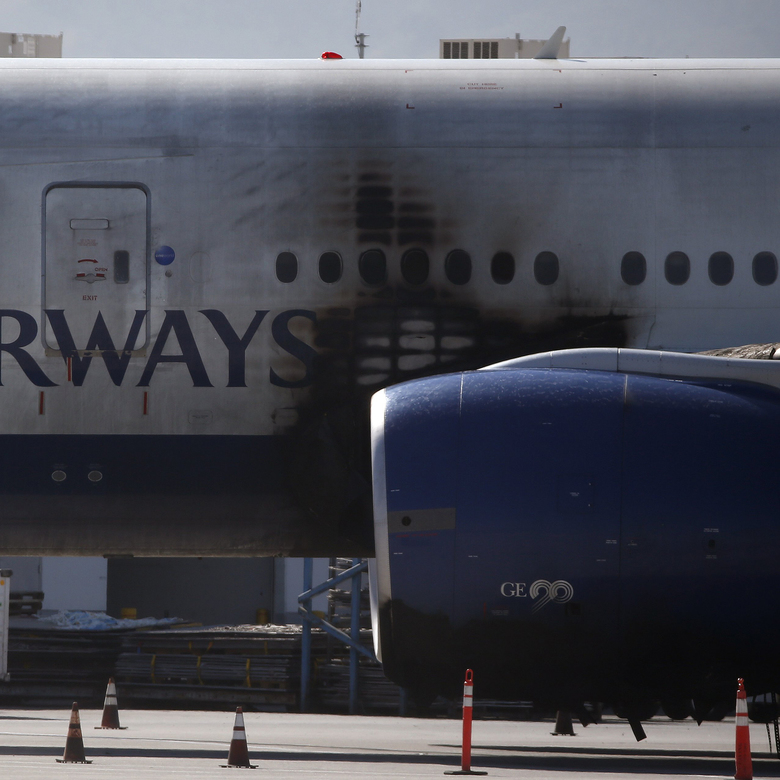
\includegraphics[scale=0.5]{animate/engine777.jpg}}\qquad
  \caption{Falla catastrófica avión 777, The Seattle Times. \cite{engine777}.}
  
\end{figure}
\end{block}
\end{frame}

\begin{frame}{Introducción}
\begin{block}{Motivación}
Falla catastrófica
\begin{figure}
  \centering
  \subfloat{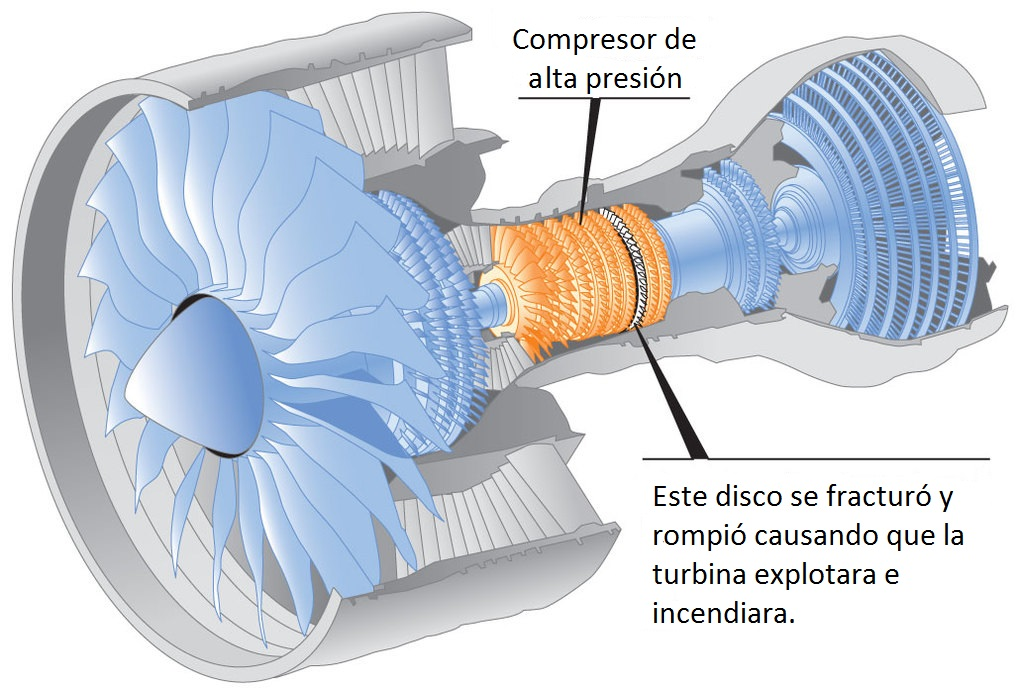
\includegraphics[scale=0.25]{animate/compressor-il-1020x688.jpg}}\qquad
  \caption{Falla catastrófica avión 777, The Seattle Times. (Imagen modificada \cite{engine777}).}
  
\end{figure}
\end{block}
\end{frame}



\begin{frame}{Introducción}

\begin{block}{Objetivo general}

Encontrar la mejor opción de red neuronal recurrente convolucional para la estimación de RUL en un sistema mecánico.
\end{block}
   
\end{frame}

\begin{frame}{Introducción}


\begin{block}{Objetivos específicos}

\begin{itemize}
    \item Estudiar modificación de la base de datos.
    \item Estudiar la aplicación de la Convolución en una serie de tiempo.
\end{itemize}
\end{block}
\end{frame}

\begin{frame}{Introducción}
\begin{block}{Alcances}
Programación y puesta en marcha de:


\begin{itemize}
    \item \textbf{ConvLSTM} 
    \item \textbf{ConvLSTM Codificadora-Decodificadora}
    \pause
    \item \textbf{ConvJANET} 
    \item \textbf{ConvJANET Codificadora-Decodificadora} 
\end{itemize}

\end{block}
   
\end{frame}
\section{Antecedentes}



\begin{frame}{Antecedentes, estimación de RUL}
    \begin{block}{RUL $\Rightarrow$ Serie de tiempo}
    \begin{figure}[!h]
        \centering
		\begin{tikzpicture}[scale=.85,cap=round] 
        %\includegraphics[scale=0.2]{imagenes/cuca_bn.jpg}
		%\node at (-2.5.5,5.5){\begin{tabular}{c}input image\\or input feature map\end{tabular}};
		
		\begin{scope}[
    	yshift=0,every node/.append style={
    	    yslant=0,xslant=0},yslant=0,xslant=0
    	             ]
        \fill[white,fill opacity=.9] (-4,0) rectangle (0,4.3);
        \draw[black,very thick] (-4,0) rectangle (0,4.3);
        \draw[step=5mm, black] (-4,0) grid (0,4.3);
        \end{scope}
        
        \begin{scope}[
    	yshift=0,every node/.append style={
    	    yslant=0,xslant=0},yslant=0,xslant=0
    	             ]
    	%\fill[white,fill opacity=.9] (0,0) rectangle (5,5);
    	%\draw[step=10mm, black] (1,1) grid (4,4);
    	%\draw[black,very thick] (1,1) rectangle (4,4);
    	%\draw[blue,dashed] (-4.15,-0.15) rectangle (0.15,1);
    	\draw[blue,dashed] (-4.15,1) rectangle (0.15,3.5);

        \end{scope}

		
		\draw (0,3.5) -- (3,1.25);%proyeccion 1
		\draw (0,1) -- (3,1.25);%proyeccion 1
		
		\begin{scope}[
    	yshift=0,every node/.append style={
    	    yslant=0,xslant=0},yslant=0,xslant=0
    	             ]
        \fill[white,fill opacity=.9] (3,0) rectangle (3.5,4.3);
        \draw[black,very thick] (3,0) rectangle (3.5,4.3);
        \draw[step=5mm, black] (3,0) grid (3.5,4.3);
        \end{scope}

		\node at (-6,2.5){\begin{tabular}{c}Ciclos\end{tabular}};
		\draw (-5,0) -- (-5,4.3);%
		\draw (-4.8,0) -- (-5.2,0);%
		\draw (-4.8,4.3) -- (-5.2,4.3);%
		
		\node at (-2,5){\begin{tabular}{c}Valores de sensores\end{tabular}};
		\draw (-4,4.7) -- (0,4.7);%
		\draw (-4,4.5) -- (-4,4.9);%
		\draw (0,4.5) -- (0,4.9);%
		
		
		%\node at (-2,5.5){\begin{tabular}{c}\textbf{Matriz de entrada}\end{tabular}};
		\node at (3.25,5.5){\begin{tabular}{c}RUL\end{tabular}};
        
	\end{tikzpicture}
		\caption{Relación entre una serie de tiempo y la RUL dentro del total de datos en la vida de una máquina. La linea punteda indica la serie de tiempo a la cual se le asocia una RUL.}
		\label{CNN}
\end{figure}
    \end{block}
\end{frame}



%perceptrón 
\begin{frame}{Antecedentes, estimación de RUL}
    \begin{block}{Una red neuronal puede relacionar ambas cosas,}
    \begin{figure}[htbp]
\centering
\begin{tikzpicture}[scale=.7,cap=round]
% Styles
\tikzstyle{information text}=[text badly centered] 
% The graphic
\begin{scope}
\pgfsetarrowsend{stealth'}
\pgfsetlinewidth{1pt}

%comentarios
%\draw (7.5,-1.4) -- (7.5,-.25)
%node[below=.9cm,text width=3cm,style=information text]
%{\small $w_{0}$ };


\node at (-3.5,3){\begin{tabular}{c}Entrada\end{tabular}};
\node at (-3.5,2.2){\begin{tabular}{c}de datos\end{tabular}};


\draw (5.5,3) -- (7.7,3)
node[below=.9cm,text width=3cm, style=information text]
{};
\draw (9.3,3) -- (11,3)
node[below=.9cm,text width=3cm, style=information text]
{};
\end{scope}

% draw the nodes

\foreach \x in {-2}
\foreach \y in {-1,0,1,2,3,4,5,6,7} {
\draw (\x,\y) circle (0.1cm);
}

\foreach \x in {4.7}
\foreach \y in {3} {
\draw (\x,\y) circle (0.7cm);
}

\foreach \x in {8.5}
\foreach \y in {3} {
\draw (\x,\y) circle (0.7cm);
}

\draw (4.7,4.7) -- (4.7,4.7)
node[below=.9cm,text width=3cm,style=information text]
{\semihuge $\sum$ };

\draw (8.5,4.7) -- (8.5,4.7)
node[below=.9cm,text width=3cm,style=information text]
{\huge $\sigma$ };

\draw (10.5,3.7)
node[below=.9cm,text width=3cm,style=information text]
{\small Estimación };

% we add the lines for the nodes starting in y 2,3, and 4

\foreach \xa / \xb in {4.4 / -1.9}
\foreach \ya / \yb in {3/-1,3/0,3/1,3/2,3/4,3/5,3/6,3/7} {
\draw (\xa,\ya) -- (\xb,\ya);
\draw (\xa,\ya) -- (\xb,\yb);
}



\end{tikzpicture}
\caption[]%
{Flujo de información y estructura típica de un Perceptrón. \cite{NN}.}
\label{F:Perceptron}
\end{figure}

\end{block}
\end{frame}

\begin{frame}{Antecedentes, redes neuronales}
\begin{figure}
	\centering
	\subfigure{
    		\begin{tikzpicture}
			\begin{axis}[width=5.5cm,height=4cm,ylabel=$\sigma(z)$,xlabel=$z$,ymin=0,ymax=1.25,xmin=-5,xmax=5]
				\addplot[blue,smooth] {1/(1+exp(-x))};
			\end{axis}
		\end{tikzpicture}
	}

	\subfigure{
		\begin{tikzpicture}
			\begin{axis}[width=5.5cm,height=4cm,ylabel=$\tanh(z)$,xlabel=$z$,ymin=-1.25,ymax=1.25,xmin=-5,xmax=5]
				\addplot[blue,smooth] {tanh(x)};
			\end{axis}
		\end{tikzpicture}
	}

    	
\end{figure}
\end{frame}


%MLP 1
\begin{frame}{Antecedentes, redes neuronales}

\begin{block}{Podemos unir muchos perceptrones,}

\begin{figure}

\begin{tikzpicture}[scale=.76,cap=round]
% Styles
\tikzstyle{information text}=[text badly centered] 

% draw the nodes

\foreach \x in {1}
\foreach \y in {0,1,2,3,4,5,6} {
\draw (\x,\y) circle (0.1cm);
}
\foreach \x in {16}
\foreach \y in {3} {
\draw (\x,\y) circle (0.1cm);
}
\foreach \x in {5,11}
\foreach \y in {1,2,3,4,5} {
\draw (\x,\y) circle (0.1cm);
}
% we add the lines for the nodes starting in y 2,3, and 4
\foreach \xa / \xb in {5.1 / 10.9 , 10.9 / 5.1}
\foreach \ya / \yb / \yc / \yd / \ye in {2 / 3 / 4 / 5 / 1, 3 / 4 / 5 / 1 /
2, 4 / 5 / 1 / 2 / 3} {
\draw (\xa,\ya) -- (\xb,\ya);
\draw (\xa,\ya) -- (\xb,\yb);
\draw (\xa,\ya) -- (\xb,\yc);
\draw (\xa,\ya) -- (\xb,\yd);
\draw (\xa,\ya) -- (\xb,\ye);
}
% add remaining lines from y1 to y5
\foreach \xa / \xb in {5.1 / 10.9 , 10.9 / 5.1}
\foreach \ya / \yb in {1 / 5, 5 / 1} {
\draw (\xa,\ya) -- (\xb,\ya);
\draw (\xa,\ya) -- (\xb,\yb);
}

% add remaining lines from y1 to y5
\foreach \xa / \xb in { 4.9/1.1}
\foreach \ya / \yb in {1/0,1/2,1/3,1/4,1/5,1/6,2/0,2/1,2/3,2/4,2/5,2/6,3/0,3/1,3/2,3/4,3/5,3/6,
4/0,4/1,4/2,4/,4/5,4/6,5/0,5/1,5/2,5/3,5/4,5/6} {
\draw (\xa,\ya) -- (\xb,\ya);
\draw (\xa,\ya) -- (\xb,\yb);
}

% add remaining lines from y1 to y5
\foreach \xa / \xb in { 15.9 / 11.1}
\foreach \ya / \yb in {3/1,3/2,3/3,3/4,3/5} {
\draw (\xa,\ya) -- (\xb,\ya);
\draw (\xa,\ya) -- (\xb,\yb);
}

\node at (-0.3,3){\begin{tabular}{c}Entrada\end{tabular}};
\node at (-0.3,2.2){\begin{tabular}{c}de datos\end{tabular}};
\node at (15.5,1.8){\begin{tabular}{c}Estimación\end{tabular}};


\end{tikzpicture}
\caption{Perceptrón de múltiples capas para regresión logística.}
\label{fig:MLP}

\end{figure}
\end{block}

\end{frame}




%MLP 0
\begin{frame}{Antecedentes, redes neuronales}

\begin{figure}

\begin{tikzpicture}[scale=.8,cap=round]
% Styles
\tikzstyle{information text}=[text badly centered] 

% draw the nodes

\foreach \x in {1}
\foreach \y in {0,1,2,3,4,5,6} {
\draw (\x,\y) circle (0.1cm);
}
\foreach \x in {16}
\foreach \y in {3} {
\draw (\x,\y) circle (0.1cm);
}
\foreach \x in {5,11}
\foreach \y in {1,2,3,4,5} {
\draw (\x,\y) circle (0.1cm);
}
%fill neuron
\draw (5,2) circle (0.1cm);
\foreach \x in {11}
\foreach \y in {1,2,3,4,5} {
\draw (\x,\y) circle (0.1cm);
}




\node at (-0.3,3){\begin{tabular}{c}Entrada\end{tabular}};
\node at (-0.3,2.2){\begin{tabular}{c}de datos\end{tabular}};
\node at (15.5,1.8){\begin{tabular}{c}Estimación\end{tabular}};



\end{tikzpicture}


\end{figure}

\end{frame}


%MLP 1
\begin{frame}{Antecedentes, redes neuronales}

\begin{figure}

\begin{tikzpicture}[scale=.8,cap=round]
% Styles
\tikzstyle{information text}=[text badly centered] 

% draw the nodes

\foreach \x in {1}
\foreach \y in {0,1,2,3,4,5,6} {
\draw (\x,\y) circle (0.1cm);
}
\foreach \x in {16}
\foreach \y in {3} {
\draw (\x,\y) circle (0.1cm);
}
\foreach \x in {5,11}
\foreach \y in {1,2,3,4,5} {
\draw (\x,\y) circle (0.1cm);
}
%fill neuron
\draw (5,2) circle (0.1cm);
\foreach \x in {11}
\foreach \y in {1,2,3,4,5} {
\draw (\x,\y) circle (0.1cm);
}


%fill path
%primera capa
\foreach \y in {0,1,2,3,4,5,6} {
\draw(1.1,\y) -- (4.9,2);
}
\foreach \y in {0,1,2,3,4,5,6} {
\draw(1.1,\y) -- (4.9,1);
}
\foreach \y in {0,1,2,3,4,5,6} {
\draw(1.1,\y) -- (4.9,5);
}


\node at (-0.3,3){\begin{tabular}{c}Entrada\end{tabular}};
\node at (-0.3,2.2){\begin{tabular}{c}de datos\end{tabular}};
\node at (15.5,1.8){\begin{tabular}{c}Estimación\end{tabular}};



\end{tikzpicture}


\end{figure}

\end{frame}

%MLP 2
\begin{frame}{Antecedentes, redes neuronales}

\begin{figure}

\begin{tikzpicture}[scale=.8,cap=round]
% Styles
\tikzstyle{information text}=[text badly centered] 

% draw the nodes

\foreach \x in {1}
\foreach \y in {0,1,2,3,4,5,6} {
\draw (\x,\y) circle (0.1cm);
}
\foreach \x in {16}
\foreach \y in {3} {
\draw (\x,\y) circle (0.1cm);
}
\foreach \x in {5,11}
\foreach \y in {1,2,3,4,5} {
\draw (\x,\y) circle (0.1cm);
}
%fill neuron
\draw (5,2) circle (0.1cm);
\foreach \x in {11}
\foreach \y in {1,2,3,4,5} {
\draw (\x,\y) circle (0.1cm);
}


%fill path
%primera capa
\foreach \y in {0,1,2,3,4,5,6} {
\draw(1.1,\y) -- (4.9,2);
}
\foreach \y in {0,1,2,3,4,5,6} {
\draw(1.1,\y) -- (4.9,1);
}
\foreach \y in {0,1,2,3,4,5,6} {
\draw(1.1,\y) -- (4.9,5);
}

%segunda capa
\foreach \y in {1,2,3,4,5} {
\draw(5.1,1) -- (10.9,\y);
}
\foreach \y in {1,2,3,4,5} {
\draw(5.1,2) -- (10.9,\y);
}
\foreach \y in {1,2,3,4,5} {
\draw(5.1,5) -- (10.9,\y);
}


\node at (-0.3,3){\begin{tabular}{c}Entrada\end{tabular}};
\node at (-0.3,2.2){\begin{tabular}{c}de datos\end{tabular}};
\node at (15.5,1.8){\begin{tabular}{c}Estimación\end{tabular}};



\end{tikzpicture}


\end{figure}

\end{frame}


%MLP 3
\begin{frame}{Antecedentes, redes neuronales}

\begin{figure}

\begin{tikzpicture}[scale=.8,cap=round]
% Styles
\tikzstyle{information text}=[text badly centered] 

% draw the nodes

\foreach \x in {1}
\foreach \y in {0,1,2,3,4,5,6} {
\draw (\x,\y) circle (0.1cm);
}
\foreach \x in {16}
\foreach \y in {3} {
\draw (\x,\y) circle (0.1cm);
}
\foreach \x in {5,11}
\foreach \y in {1,2,3,4,5} {
\draw (\x,\y) circle (0.1cm);
}
%fill neuron
\draw (5,2) circle (0.1cm);
\foreach \x in {11}
\foreach \y in {1,2,3,4,5} {
\draw (\x,\y) circle (0.1cm);
}


%fill path
%primera capa
\foreach \y in {0,1,2,3,4,5,6} {
\draw(1.1,\y) -- (4.9,2);
}
\foreach \y in {0,1,2,3,4,5,6} {
\draw(1.1,\y) -- (4.9,1);
}
\foreach \y in {0,1,2,3,4,5,6} {
\draw(1.1,\y) -- (4.9,5);
}

%segunda capa
\foreach \y in {1,2,3,4,5} {
\draw(5.1,1) -- (10.9,\y);
}
\foreach \y in {1,2,3,4,5} {
\draw(5.1,2) -- (10.9,\y);
}
\foreach \y in {1,2,3,4,5} {
\draw(5.1,5) -- (10.9,\y);
}

% tercera capa
\foreach \xa / \xb in { 15.9 / 11.1}
\foreach \ya / \yb in {3/1,3/2,3/3,3/4,3/5} {

\draw (\xa,\ya) -- (\xb,\yb);
}

\node at (-0.3,3){\begin{tabular}{c}Entrada\end{tabular}};
\node at (-0.3,2.2){\begin{tabular}{c}de datos\end{tabular}};
\node at (15.5,1.8){\begin{tabular}{c}Estimación\end{tabular}};



\end{tikzpicture}


\end{figure}

\end{frame}
%%%%%%%%%%%%%%
%%%%%%%%%%%%%%
%%%%%%%%%%%%%%


\begin{frame}{Antecedentes, redes neuronales}
    \begin{block}{Retropropagación \cite{BPTT},}
    \begin{figure}
        \centering
        \begin{tikzpicture}[scale=0.85]
        
\begin{axis}[
    hide axis,
    colormap/cool,
]
\addplot3[
    mesh,
    samples=50,
    domain=-8:8,
]
{ cos(deg(sqrt(x^2+y^2)))*sin(deg(sqrt(x^2+y^2)))/sqrt(x^2+y^2)};
\end{axis}
\end{tikzpicture}
        \caption{Superficie creada por distintas posibilidades de pesos y un error determinado.}
        \label{fig:surface}
    \end{figure}
    \end{block}
    
    \begin{block}{Los optimizadores ajustan los pesos}
    \begin{itemize}
    \item Cuanto se ajusta, $\bigtriangleup w_{ij} = -\eta \frac{\partial E_{n}}{\partial w_{ij}}$.
    \item Cómo se ajusta, $w_{ij} = w_{ij} + \bigtriangleup w_{ij}$.
    \end{itemize}
    \end{block}
\end{frame}



\begin{frame}{Antecedentes, redes neuronales}
    \begin{block}{Redes Neuronales Convolucionales \cite{CNN},}
    \begin{figure}
        
        \centering
		\begin{tikzpicture}[scale=0.9]
		
		\begin{scope}[
    	yshift=0,every node/.append style={
    	    yslant=0,xslant=0},yslant=0,xslant=0
    	             ]
        \fill[white,fill opacity=.9] (-4,0) rectangle (0,4.3);
        \draw[black,very thick] (-4,0) rectangle (0,4.3);
        \draw[step=5mm, black] (-4,0) grid (0,4.3);
        \end{scope}
        
        \begin{scope}[
    	yshift=0,every node/.append style={
    	    yslant=0,xslant=0},yslant=0,xslant=0
    	             ]
    	%\fill[white,fill opacity=.9] (0,0) rectangle (5,5);
    	%\draw[step=10mm, black] (1,1) grid (4,4);
    	%\draw[black,very thick] (1,1) rectangle (4,4);
    	%\draw[blue,dashed] (-4.15,-0.15) rectangle (0.15,1);
    	%\draw[blue,dashed] (-4.15,3.5) rectangle (0.15,4.5);

        \end{scope}
    	
        	
	
		%\draw (-3,1) -- (0,1) -- (0,4.3) -- (-3,4.3) -- (-3,1);%imagen
		
	    \draw [fill=black,opacity=0.5,draw=black](0,3.3) -- (-0.5,3.3) -- (-0.5,4.3) -- (0,4.3) -- (0,3.3);%kernel 1
		\draw [fill=black,opacity=0.35,draw=black](-2,3) -- (-2.5,3) -- (-2.5,2) -- (-2,2) -- (-2,3);%kernel 3
		\draw [fill=black,opacity=0.5,draw=black](-1,1) -- (-1.5,1) -- (-1.5,2) -- (-1,2) -- (-1,1);%kernel 2
		
		\draw (-2.,3) -- (4,3.25);%proyeccion 1
		\draw (-2.,2.0) -- (4,3.25);%proyeccion 1

		\draw (0,4.3) -- (4.75,4.3);%proyeccion 3
		\draw (0,3.3) -- (4.75,4.3);%proyeccion 3
		
		\draw (-1.,2) -- (1.5,1.25);%proyeccion 2
		\draw (-1.,1.0) -- (1.5,1.25);%proyeccion 2
		
		\node at (-2,5){\begin{tabular}{c}Matriz de entrada\end{tabular}};
		\node at (3.25,5.5){\begin{tabular}{c}Salida\end{tabular}};
		\node at (3.25,5){\begin{tabular}{c}mapa de características\end{tabular}};
		\node at (8.5,5.5){\begin{tabular}{c}Capa total-conectada\end{tabular}};
		\node at (8.5,5){\begin{tabular}{c}junto a la estimación\end{tabular}};
		
		
		
		\draw[fill=black,opacity=0.1,draw=black] (3.5,2.5) -- (5.5,2.5) -- (5.5,4.5) -- (3.5,4.5) -- (3.5,2.5)--(3,2);
		\draw[fill=black,opacity=0.1,draw=black] (3,2) -- (5,2) -- (5,4) -- (3,4) -- (3,2);
		\draw[fill=black,opacity=0.1,draw=black] (2.5,1.5) -- (4.5,1.5) -- (4.5,3.5) -- (2.5,3.5) -- (2.5,1.5);
		\draw[fill=black,opacity=0.2,draw=black] (2,1) -- (4,1) -- (4,3) -- (2,3) -- (2,1);
		\draw[fill=black,opacity=0.3,draw=black] (1.5,0.5) -- (3.5,0.5) -- (3.5,2.5) -- (1.5,2.5) -- (1.5,0.5);
		\draw[fill=black,opacity=0.4,draw=black] (1,0) -- (3,0) -- (3,2) -- (1,2) -- (1,0);
		
		
        \draw (4.75,4.3) circle (0.05cm);
        \draw (4,3.25) circle (0.05cm);
        \draw (1.5,1.25) circle (0.05cm);
        
        %full-connected layer
        \draw (4.75,4.3) circle (0.05cm);
        \draw (4,3.25) circle (0.05cm);
        \draw (1.5,1.25) circle (0.05cm);
        
        \draw (8.5,2.25) circle (0.1cm);
        
        \draw (8,3.5) circle (0.1cm);
        \draw (7.5,3) circle (0.1cm);
        \draw (7,2.5) circle (0.1cm);
        \draw (6.5,2) circle (0.1cm);
        \draw (6,1.5) circle (0.1cm);
        \draw (5.5,1) circle (0.1cm);
        
        %conections in first nodo
        \draw (5.5,4.5) -- (7.9,3.5);
        \draw (5,4) -- (7.9,3.5);
        \draw (4.5,3.5) -- (7.9,3.5);
        \draw (4,3) -- (7.9,3.5);
        \draw (3.5,2.5) -- (7.9,3.5);
        \draw (3,2) -- (7.9,3.5);
        
        
        
        %conections in second nodo
        \draw (5.5,4.5) -- (7.4,3);
        \draw (5,4) -- (7.4,3);
        \draw (4.5,3.5) -- (7.4,3);
        \draw (4,3) -- (7.4,3);
        \draw (3.5,2.5) -- (7.4,3);
        \draw (3,2) -- (7.4,3);
        
        %conections in third nodo
        \draw (5.5,4.5) -- (6.9,2.5);
        \draw (5,4) -- (6.9,2.5);
        \draw (4.5,3.5) -- (6.9,2.5);
        \draw (4,3) -- (6.9,2.5);
        \draw (3.5,2.5) -- (6.9,2.5);
        \draw (3,2) -- (6.9,2.5);
        
        %conections in fourth nodo
        \draw (5.5,4.5) -- (6.4,2);
        \draw (5,4) -- (6.4,2);
        \draw (4.5,3.5) -- (6.4,2);
        \draw (4,3) -- (6.4,2);
        \draw (3.5,2.5) -- (6.4,2);
        \draw (3,2) -- (6.4,2);
        
        %conections in fifth nodo
        \draw (5.5,4.5) -- (5.9,1.5);
        \draw (5,4) -- (5.9,1.5);
        \draw (4.5,3.5) -- (5.9,1.5);
        \draw (4,3) -- (5.9,1.5);
        \draw (3.5,2.5) -- (5.9,1.5);
        \draw (3,2) -- (5.9,1.5);
        
        
        %conections in sixth nodo
        \draw (5.5,4.5) -- (5.4,1);
        \draw (5,4) -- (5.4,1);
        \draw (4.5,3.5) -- (5.4,1);
        \draw (4,3) -- (5.4,1);
        \draw (3.5,2.5) -- (5.4,1);
        \draw (3,2) -- (5.4,1);
        
        \draw (5.5,2.5) -- (5.4,1);
        \draw (5,2) -- (5.4,1);
        \draw (4.5,1.5) -- (5.4,1);
        \draw (4,1) -- (5.4,1);
        \draw (3.5,0.5) -- (5.4,1);
        \draw (3,0) -- (5.4,1);
        
        %conections in last nodo
        \draw (5.6,1) -- (8.4,2.25);
        \draw (6.1,1.5) -- (8.4,2.25);
        \draw (6.6,2) -- (8.4,2.25);
        \draw (7.1,2.5) -- (8.4,2.25);
        \draw (7.6,3) -- (8.4,2.25);
        \draw (8.1,3.5) -- (8.4,2.25);
        
        
	\end{tikzpicture}
	\caption{Modelo estándar de aplicación de redes neuronales convolucionales.}
        \label{fig:CNN}
    \end{figure}
    
    \end{block}
\end{frame}


\begin{frame}{Antecedentes, redes neuronales}
    \begin{block}{Redes neuronales recurrentes (\cite{RNN1} y \cite{RNN2}),}
    \begin{figure}[!h]

   \begin{tikzpicture}[scale=.5]
   \begin{scope}
   \pgfsetarrowsend{stealth'}
   \pgfsetlinewidth{0.1pt}
   %first RNN
   \draw (2,-1.4) -- (2,0.2);
   \draw (2,1.7) -- (2,3.3);
   \draw (2,1.7) .. controls +(2,1.25) and +(2,-0.8)..  (2.1,0.2);
   
   %unroled 1
   \draw (6,-1.4) -- (6,0.2);
   \draw (6,1.7) -- (6,3.3);
   \draw (6.75,1) -- (9.25,1);
   
   %unroled 2
   \draw (10,-1.4) -- (10,0.2);
   \draw (10,1.7) -- (10,3.3);
   \draw (10.75,1) -- (13.25,1);
   
   %unroled 
   \draw (14,-1.4) -- (14,0.2);
   \draw (14,1.7) -- (14,3.3);
   \draw (14.75,1) -- (15.15,1);
\end{scope}
    ;
	%first RNN
	\draw[fill=black,opacity=0.4,draw=black] (2,1) circle (0.7cm);
	\draw (4.4,3.25) -- (4.4,3.25)%(x+2.4,y+1.05)
	node[below=.9cm,text width=3cm,style=information text]
	{\scriptsize RNN };
	\draw (4.7,0.2) -- (4.7,0.2)%cambiar 2.7 (2.7+x,y+1.2)
	node[below=.9cm,text width=3cm,style=information text]
	{\small $x^{(t)}$ };
	\draw (4.7,6.5) -- (4.7,6.8)%cambiar 2.7 (2.7+x,y+1.5)
	node[below=.9cm,text width=3cm,style=information text]
	{\small $y^{(t)}$ };
	\draw (5.5,5) -- (5.5,5)
	node[below=.9cm,text width=3cm,style=information text]
	{\small $h^{(t)}$ };
	\draw (5.5,1.9) -- (5.5,1.9)
	node[below=.9cm,text width=3cm,style=information text]
	{\small $h^{(t-1)}$ };
	\draw (4.7,-1) -- (4.7,-1)%(x+2.7,y)
	node[below=.9cm,text width=3cm,style=information text]
	{\small $(a)$ };
	\draw (2,3.5) circle (0.1cm);
	\draw (2,-1.5) circle (0.1cm);
	\draw[fill=white,opacity=1,draw=black] (3.55, 1) circle (0.1cm);
	
	%unroled 1
	\draw[fill=black,opacity=0.3,draw=black] (6,1) circle (0.7cm);
	\draw (8.4,3.25) -- (8.4,3.25)
	node[below=.9cm,text width=3cm,style=information text]
	{\scriptsize RNN };
	\draw (10.5, 2.8) -- (10.5, 2.8)
	node[below=.9cm,text width=3cm,style=information text]
	{\small $h^{(1)}$ };
	\draw (8.7,0.2) -- (8.7,0.2)
	node[below=.9cm,text width=3cm,style=information text]
	{\small $x^{(1)}$ };
	\draw (8.7,6.8) -- (8.7,6.8)
	node[below=.9cm,text width=3cm,style=information text]
	{\small $y^{(1)}$ };
	\draw (6,3.5) circle (0.1cm);
	\draw (6,-1.5) circle (0.1cm);
	\draw[fill=white,opacity=1,draw=black] (8, 1) circle (0.1cm);
	
	
	%unroled 2
	\draw[fill=black,opacity=0.2,draw=black] (10,1) circle (0.7cm);
	\draw (12.4,3.25) -- (12.4,3.25)
	node[below=.9cm,text width=3cm,style=information text]
	{\scriptsize RNN };
	\draw (14.5, 2.8) -- (14.5, 2.8)
	node[below=.9cm,text width=3cm,style=information text]
	{\small $h^{(2)}$ };
	\draw (12.7,0.2) -- (12.7,0.2)
	node[below=.9cm,text width=3cm,style=information text]
	{\small $x^{(2)}$ };
	\draw (12.7,6.8) -- (12.7,6.8)
	node[below=.9cm,text width=3cm,style=information text]
	{\small $y^{(2)}$ };
	\draw (12.7,-1) -- (12.7,-1)
	node[below=.9cm,text width=3cm,style=information text]
	{\small $(b)$ };
	\draw (10,3.5) circle (0.1cm);
	\draw (10,-1.5) circle (0.1cm);
	\draw[fill=white,opacity=1,draw=black] (12, 1) circle (0.1cm);
	
	%unroled 3
	\draw[fill=black,opacity=0.1,draw=black] (14,1) circle (0.7cm);
	\draw (16.4,3.25) -- (16.4,3.25)
	node[below=.9cm,text width=3cm,style=information text]
	{\scriptsize RNN };
	\draw (17.8, 2.8) -- (17.8, 2.8)
	node[below=.9cm,text width=3cm,style=information text]
	{\small $h^{(3)}$ };
	\draw (16.7,0.2) -- (16.7,0.2)
	node[below=.9cm,text width=3cm,style=information text]
	{\small $x^{(3)}$ };
	\draw (16.7,6.8) -- (16.7,6.8)
	node[below=.9cm,text width=3cm,style=information text]
	{\small $y^{(3)}$ };
	\draw (14,3.5) circle (0.1cm);
	\draw (14,-1.5) circle (0.1cm);
	\draw[fill=white,opacity=1,draw=black] (15.3, 1) circle (0.1cm);
	

	
\end{tikzpicture}
    \caption{Célula de red recurrente. Grafo cíclico tipico $(a)$ que puede ser desplagado en $(b)$ como grafo acíclico. }
    \label{fig:RNN}
\end{figure}

    \end{block}
\end{frame}
%%%%%%%%%%%%%%
%%%%%%%%%%%%%%
%%%%%%%%%%%%%%


\begin{frame}{Antecedentes, redes neuronales}
    \begin{block}{Redes neuronales recurrentes, LSTM \cite{LSTM},}
    \begin{figure}
    \centering
   \begin{tikzpicture}[scale=.6]
   \begin{scope}
   \pgfsetarrowsend{stealth'}
   \pgfsetlinewidth{0.1pt}
   
   
   %unroled 1
   \draw (6,-1.4) -- (6,0.2);
   \draw (6,1.7) -- (6,3.3);
   
   
   %unroled 2
   \draw (10,-1.4) -- (10,0.2);
   \draw (10,1.7) -- (10,3.3);
   %\draw (10.75,1) -- (13.25,1);
   
   %unroled 
   \draw (14,-1.4) -- (14,0.2);
   \draw (14,1.7) -- (14,3.3);
   %\draw (14.75,1) -- (15.15,1);
\end{scope}
    ;
	
	
	%unroled 1
	\draw[fill=black,opacity=0.3,draw=black] (6,1) circle (0.7cm);
	\draw (7.85,2.9) -- (7.85,2.9)
	node[below=.9cm,text width=3cm,style=information text]
	{\scriptsize LSTM };
	
	
	\draw (8.2,-0.2) -- (8.2,-0.2)
	node[below=.9cm,text width=3cm,style=information text]
	{\small $x^{(1)}$ };
	\draw (8.2,6.5) -- (8.2,6.5)
	node[below=.9cm,text width=3cm,style=information text]
	{\small $y^{(1)}$ };
	\draw (6,3.5) circle (0.1cm);
	\draw (6,-1.5) circle (0.1cm);
	
	%flecha de transferencia
	
	\begin{scope}
   \pgfsetarrowsend{stealth'}
   \pgfsetlinewidth{0.1pt}
	\draw (6.75,1.3) -- (9.25,1.3);
	\draw (6.75,0.7) -- (9.25,0.7);
	
	\end{scope}
	\draw[fill=white,opacity=1,draw=black] (8, 1.3) circle (0.1cm);%circulo tranferencia
	\draw[fill=white,opacity=1,draw=black] (8, 0.7) circle (0.1cm);%circulo tranferencia
	
	%informacion tranferida
	\draw (10, 2) -- (10, 2)
	node[below=.9cm,text width=3cm,style=information text]
	{\small $h^{(1)}$ };
	\draw (10, 4.1) -- (10, 4.1)
	node[below=.9cm,text width=3cm,style=information text]
	{\small $c^{(1)}$ };
	
	
	%unroled 2
	\draw[fill=black,opacity=0.2,draw=black] (10,1) circle (0.7cm);
	\draw (11.85,2.9) -- (11.85,2.9)
	node[below=.9cm,text width=3cm,style=information text]
	{\scriptsize LSTM };
	
	\draw (12.2,-0.2) -- (12.2,-0.2)
	node[below=.9cm,text width=3cm,style=information text]
	{\small $x^{(2)}$ };
	\draw (12.2,6.5) -- (12.2,6.5)
	node[below=.9cm,text width=3cm,style=information text]
	{\small $y^{(2)}$ };
	
	\draw (10,3.5) circle (0.1cm);
	\draw (10,-1.5) circle (0.1cm);
	%\draw[fill=white,opacity=1,draw=black] (12, 1) circle (0.1cm);
	
	%flecha de transferencia
	
	\begin{scope}
   \pgfsetarrowsend{stealth'}
   \pgfsetlinewidth{0.1pt}
	\draw (10.75,1.3) -- (13.25,1.3);
	\draw (10.75,0.7) -- (13.25,0.7);
	
	\end{scope}
	\draw[fill=white,opacity=1,draw=black] (12, 1.3) circle (0.1cm);%circulo tranferencia
	\draw[fill=white,opacity=1,draw=black] (12, 0.7) circle (0.1cm);%circulo tranferencia
	
	%informacion tranferida
	\draw (14, 2) -- (14, 2)
	node[below=.9cm,text width=3cm,style=information text]
	{\small $h^{(2)}$ };
	\draw (14, 4.1) -- (14, 4.1)
	node[below=.9cm,text width=3cm,style=information text]
	{\small $c^{(2)}$ };
	
	%unroled 3
	\draw[fill=black,opacity=0.1,draw=black] (14,1) circle (0.7cm);
	\draw (15.85,2.9) -- (15.85,2.9)
	node[below=.9cm,text width=3cm,style=information text]
	{\scriptsize LSTM };
	
	\draw (16.2,-0.2) -- (16.2,-0.2)
	node[below=.9cm,text width=3cm,style=information text]
	{\small $x^{(3)}$ };
	\draw (16.2,6.5) -- (16.2,6.5)
	node[below=.9cm,text width=3cm,style=information text]
	{\small $y^{(3)}$ };
	\draw (14,3.5) circle (0.1cm);
	\draw (14,-1.5) circle (0.1cm);
	
	
	%flecha de transferencia
	
	\begin{scope}
   \pgfsetarrowsend{stealth'}
   \pgfsetlinewidth{0.1pt}
	\draw (14.75,1.3) -- (15.15,1.3);
	\draw (14.75,0.7) -- (15.15,0.7);
	
	\end{scope}
	\draw[fill=white,opacity=1,draw=black] (15.3, 1.3) circle (0.1cm);%circulo tranferencia
	\draw[fill=white,opacity=1,draw=black] (15.3, 0.7) circle (0.1cm);%circulo tranferencia
	
	%informacion tranferida
	\draw (17.8, 2) -- (17.8, 2)
	node[below=.9cm,text width=3cm,style=information text]
	{\small $h^{(3)}$ };
	\draw (17.8, 4.1) -- (17.8, 4.1)
	node[below=.9cm,text width=3cm,style=information text]
	{\small $c^{(3)}$ };
	
	

	
\end{tikzpicture}
    \caption{Flujo de información en célula LSTM. }
    \label{fig:RNN}
\end{figure}

    \end{block}
\end{frame}


\begin{frame}{Antecedentes, redes neuronales}
    \begin{block}{Redes neuronales recurrentes, JANET \cite{janet},}
    \begin{figure}
   \centering
   \begin{tikzpicture}[scale=.6]
   \begin{scope}
   \pgfsetarrowsend{stealth'}
   \pgfsetlinewidth{0.1pt}
   
   
   %unroled 1
   \draw (6,-1.4) -- (6,0.2);
   
   \draw (6.75,1) -- (9.25,1);
   
   %unroled 2
   \draw (10,-1.4) -- (10,0.2);
   
   \draw (10.75,1) -- (13.25,1);
   
   %unroled 
   \draw (14,-1.4) -- (14,0.2);
   
   \draw (14.75,1) -- (15.15,1);
\end{scope}
    ;
	
	
	%unroled 1
	\draw[fill=black,opacity=0.3,draw=black] (6,1) circle (0.7cm);
	\draw (7.9,2.9) -- (7.9,2.9)
	node[below=.9cm,text width=3cm,style=information text]
	{\tiny JANET };
	\draw (10, 2.3) -- (10, 2.3)
	node[below=.9cm,text width=3cm,style=information text]
	{\small $c^{(1)}$ };
	\draw (8.2,-0.2) -- (8.2,-0.2)
	node[below=.9cm,text width=3cm,style=information text]
	{\small $x^{(1)}$ };
	
	
	\draw (6,-1.5) circle (0.1cm);
	\draw[fill=white,opacity=1,draw=black] (8, 1) circle (0.1cm);
	
	
	%unroled 2
	\draw[fill=black,opacity=0.2,draw=black] (10,1) circle (0.7cm);
	\draw (11.9,2.9) -- (11.9,2.9)
	node[below=.9cm,text width=3cm,style=information text]
	{\tiny JANET};
	\draw (14, 2.3) -- (14, 2.3)
	node[below=.9cm,text width=3cm,style=information text]
	{\small $c^{(2)}$ };
	\draw (12.2,-0.2) -- (12.2,-0.2)
	node[below=.9cm,text width=3cm,style=information text]
	{\small $x^{(2)}$ };
	
	
	
	\draw (10,-1.5) circle (0.1cm);
	\draw[fill=white,opacity=1,draw=black] (12, 1) circle (0.1cm);
	
	%unroled 3
	\draw[fill=black,opacity=0.1,draw=black] (14,1) circle (0.7cm);
	\draw (15.9,2.9) -- (15.9,2.9)
	node[below=.9cm,text width=3cm,style=information text]
	{\tiny JANET};
	\draw (17.3, 2.3) -- (17.3, 2.3)
	node[below=.9cm,text width=3cm,style=information text]
	{\small $c^{(3)}$ };
	\draw (16.2,-0.2) -- (16.2,-0.2)
	node[below=.9cm,text width=3cm,style=information text]
	{\small $x^{(3)}$ };
	
	
	\draw (14,-1.5) circle (0.1cm);
	\draw[fill=white,opacity=1,draw=black] (15.3, 1) circle (0.1cm);
	

	
\end{tikzpicture}
    \caption{Flujo de información en JANET. }
    \label{fig:RNN}
\end{figure}

    \end{block}
\end{frame}

\begin{frame}{Antecedentes, redes neuronales recurrentes convolucionales}
    \begin{block}{Aplicable de forma directa similar a una CNN,}
    \begin{figure}
        \centering
        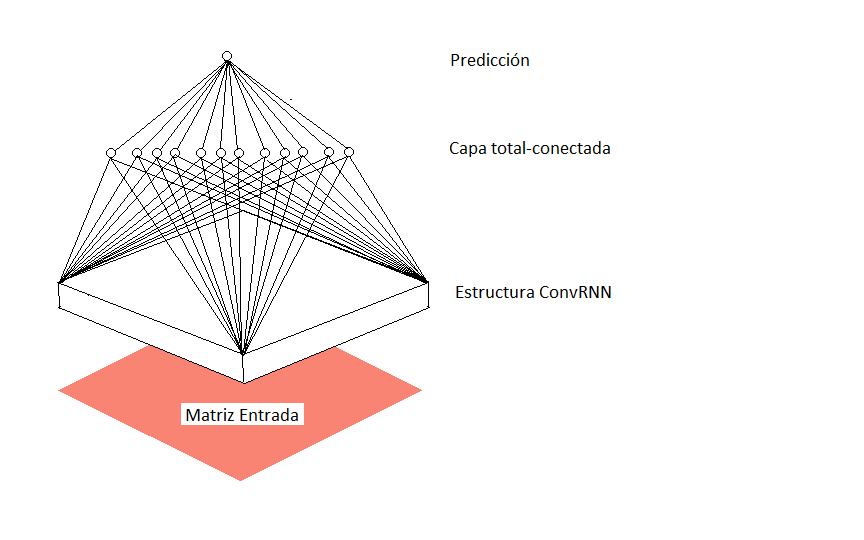
\includegraphics[scale=0.4]{animate/conv_lstm.png}
        \caption{Aplicación directa de una ConvRNN para la predicción.}
        \label{fig:convrnn}
    \end{figure}
    \end{block}
\end{frame}

\begin{frame}{Antecedentes, redes neuronales recurrentes convolucionales}
    \begin{block}{Como Codificadora-Decodificadora (\cite{convlstm}, \cite{E-D1} y \cite{E-D2}),}
    \begin{figure}
        \centering
        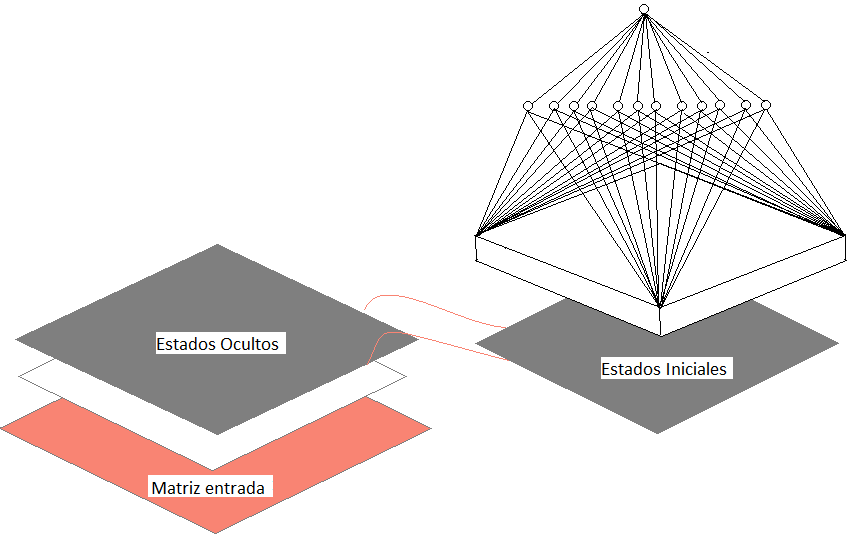
\includegraphics[scale=0.4]{animate/Codificador-Decodificador.png}
        \caption{Aplicación de ConvRNN como Codificadora-Decodificadora para la predicción.}
        \label{fig:my_label}
    \end{figure}
    \end{block}
\end{frame}

\begin{frame}{Antecedentes, Base de datos}
\begin{block}{Turbofan}

\begin{figure}[!h]
		\centering
		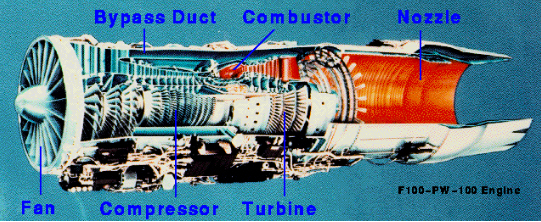
\includegraphics[scale=0.5]{animate/turbofan31.png}
		\caption{Descripción de partes de un turbofan donde se especifica el ducto de bypass. \cite{bypass_nasa}. }
		\label{logofcfm}
	\end{figure}
\end{block}
\end{frame}
%foto turbofan: https://www.grc.nasa.gov/www/k-12/Missions/Jim/Project2_act.htm


\begin{frame}{Antecedentes, Base de datos}
\begin{block}{C-MAPSS \cite{metricas-rmse}}
\begin {itemize}
    \item Datos como velocidad, presión, temperatura, etc.
    \pause
    \item Ruido blanco.
    \pause
    \item Operación y fallas.
    \pause
    \item Cantidad de datos.
\end {itemize}
\end{block}
\end{frame}

\begin{frame}{Antecedentes, Medición de exactitud}
    \begin{figure}
        \centering
        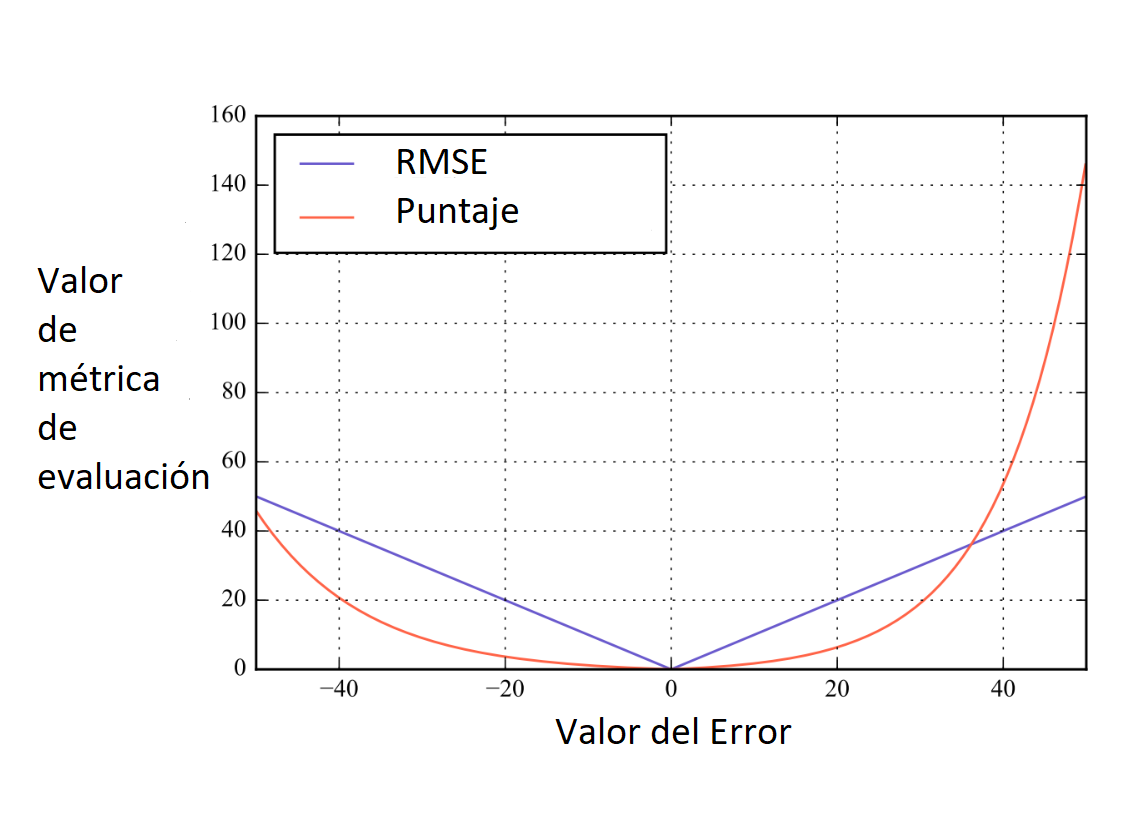
\includegraphics[scale=0.3]{animate/error_metricas_evaluacion.png}
        \caption{Asignación de puntaje y exactitud de un modelo según su error. \cite{metricas-rmse}.}
        \label{fig:rmse-score}
    \end{figure}
\end{frame}


\section{Metodología}

\begin{frame}{Metodología, Uso de bases de datos}
\begin{figure}
    
    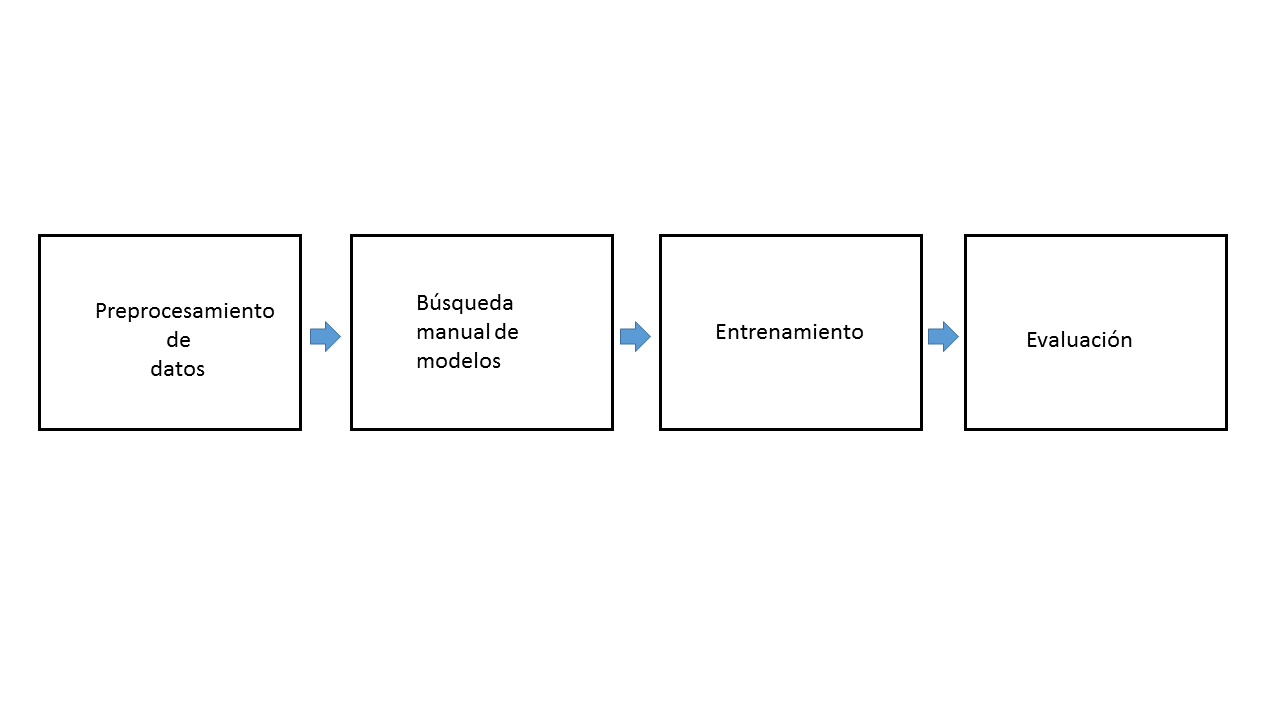
\includegraphics[scale=0.4]{animate/Presentacion1.png}
    \caption{Procedimientos a seguir en la metodología.}
    \label{fig:my_label}
\end{figure}
\end{frame}

\begin{frame}{Metodología, Preprocesamiento de datos}
    \begin{figure}
        \centering
        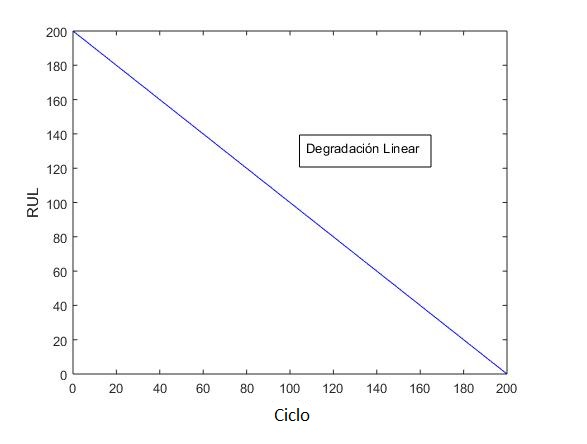
\includegraphics[scale=0.55]{animate/sin_modificar_RUL.jpg}
        \caption{RULs de bases de datos sin modificar.}
        \label{fig:my_label}
    \end{figure}
\end{frame}


\begin{frame}{Metodología, Preprocesamiento de datos}
    \begin{figure}
        \centering
        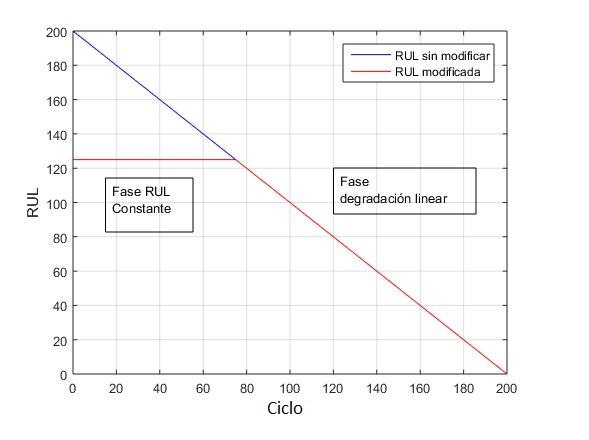
\includegraphics[scale=0.55]{animate/RUL_modificada.jpg}
        \caption{RULs de bases de datos modificadas.}
        \label{fig:my_label}
    \end{figure}
\end{frame}


\section{Resultados y Discusión}
\begin{frame}{Resultados, Histogramas}
\begin{figure}
    \centering
    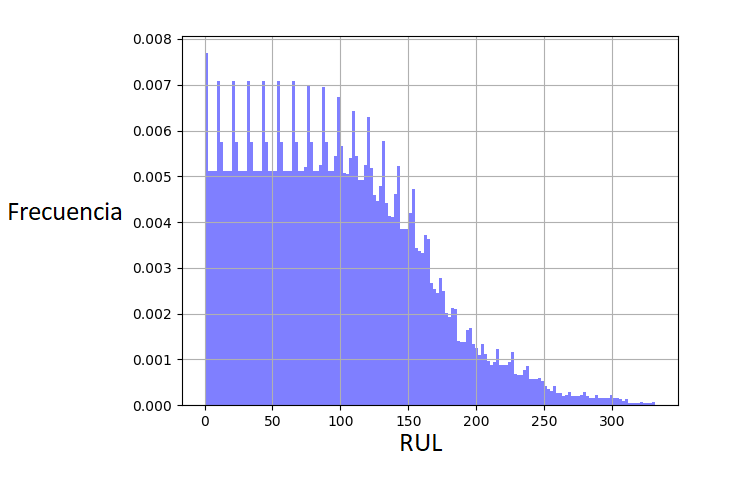
\includegraphics[scale=0.5]{animate/histograma_FD001(mejorado).png}
    \caption{Histograma de RULs sobre set FD001.}
    \label{fig:hist1}
\end{figure}
\end{frame}

\begin{frame}{Resultados, Mejores modelos}
    \begin{figure}
        \centering
        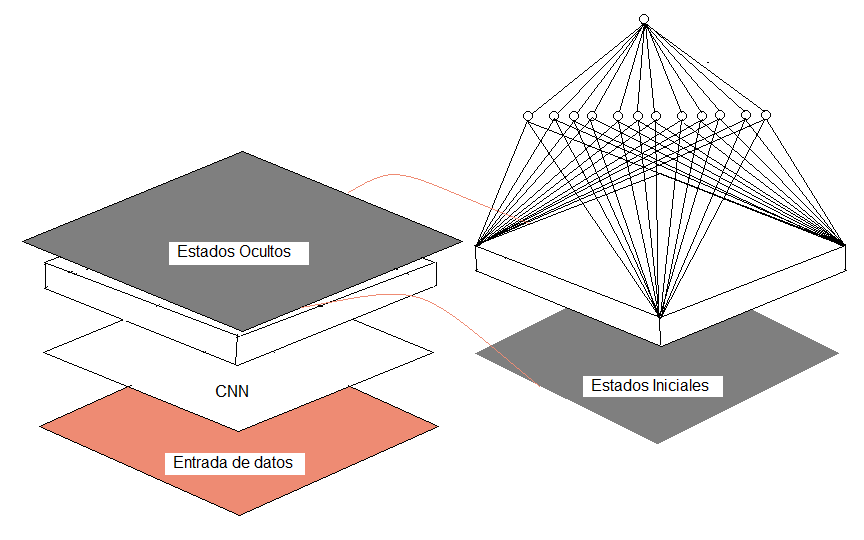
\includegraphics[scale=0.48]{animate/modelo_winer.png}
        \caption{Modelo recurrente convolucional obtenido.}
        \label{fig:my_label}
    \end{figure}
\end{frame}

\begin{frame}{Resultados}
% Please add the following required packages to your document preamble:
% \usepackage{booktabs}
% \usepackage{multirow}
\begin{table}[H]
\centering
 
\label{tab:test_FD004}
\begin{tabular}{@{}cccc@{}}
\toprule
\multirow{2}{*}{Modelo} & \multicolumn{3}{c}{FD004}                     \\ \cmidrule(l){2-4} 
                       & RMSE        & Puntaje           & Tiempo entre. (s) \\ \cmidrule(r){1-1}
ConvJANET              & 19,55  $\pm$  0,3  & {\color[HTML]{3166FF}2.259,53  +-  185,71} & {\color[HTML]{3166FF}255,40  +-  0,51}  \\
ConvJANET C-D          & {\color[HTML]{3166FF}19,15}   $\pm$   {\color[HTML]{3166FF}0,28} & 2282,23  $\pm$  226,58 & 490,95  $\pm$  0,63  \\
ConvLSTM               & {\color[HTML]{FE0000}20,75 +- 0,81} & {\color[HTML]{FE0000}2.513,57  +-  287,81} & 266,11  $\pm$  1,51  \\
ConvLSTM C-D           & 19,53  $\pm$  0,23 & 2316,28  $\pm$  180,84 & {\color[HTML]{FE0000}615,03  +-  0,65}  \\ \bottomrule
\end{tabular}
\caption{ConvLSTM, ConvJANET y sus variedades Codificadora-Decodificadora evaluadas en FD004. }
\end{table}
\pause
\begin{block}{Red convolucional profunda (estado del arte \cite{estado-arte})}
RMSE: media de 23,31 $\pm$ 0,39\\
Puntaje: media de 12.466 $\pm$ 853
\end{block}
\end{frame}

\begin{frame}{Resultados, Ajuste de ConvJANET Codificadora-Decodificadora en FD003}
%%%%%%%%%%%%%%%%%%%%%%
%ConvJANET_ED FD004
%%%%%%%%%%%%%%%%%%%%%%
%grafico cross_val vs train
%%%%%%%%%%%%%%%%%%%%%%
\begin{figure}[H]
\centering
\begin{tikzpicture}[scale=0.85]
\begin{axis}[title={},xlabel={Paso (escala 1:100)},ylabel={RMSE},xmin=0, xmax=200,ymin=0, ymax=120,xtick={0, 20, 40, 60, 80, 100, 120, 140, 160, 180, 200, 220},
ytick={0, 5, 10, 15, 20, 25, 30, 35, 40, 45, 50, 55, 60, 65, 70, 75, 80, 85, 90,100,110,120},
ymajorgrids=true,
grid style=dashed,]
\addplot[color=red,mark=triangle,]coordinates {(1,93.8872
)(11,24.6388
)(21,12.9999
)(31,10.4563
)(41,8.4857
)(51,7.8378
)(61,6.6042
)(71,6.0978
)(81,5.1937
)(91,4.6956
)(101,4.5252
)(111,3.4615
)(121,3.1987
)(131,2.9951
)(141,3.2304
)(151,2.5639
)(161,2.7364
)(171,2.6651
)(181,2.5460
)(191,2.4033
)(200,4.1715
)};
\addlegendentry{Set de entrenamiento}
\addplot[color=blue,mark=triangle,]coordinates {(1,94.8226
)(11,24.6045
)(21,12.2327
)(31,10.3775
)(41,8.9068
)(51,7.6617
)(61,6.9687
)(71,6.5419
)(81,5.6088
)(91,5.3066
)(101,5.2221
)(111,4.6524
)(121,4.2436
)(131,3.8091
)(141,4.2439
)(151,3.8358
)(161,3.6080
)(171,3.7765
)(181,3.4179
)(191,3.5491
)(200,4.5634
)};
\addlegendentry{Set de validación}
\end{axis}
\end{tikzpicture}
\caption{Exactitud en sets de validación y entrenamiento en cada paso de entrenamiento para ConvJANET Codificadora-Decodificadora en FD003.}
\label{fig:Histogram_FD003}
\end{figure}
    
\end{frame}
%
\begin{frame}{Resultados, Predicciones de ConvJANET Codificadora-Decodificadora en FD003}
\begin{figure}[H]
\centering
\begin{tikzpicture}[scale=0.85]
\begin{axis}[title={},xlabel={Ejemplos de turbofanes (orden decreciente de RULs)},ylabel={RUL},xmin=0, xmax=100,ymin=0, ymax=130,xtick={0, 10, 20, 30, 40, 50, 60, 70, 80, 90, 100},
ytick={0, 5, 10, 15, 20, 25, 30, 35, 40, 45, 50, 55, 60, 65, 70, 75, 80, 85, 90,100,110,120},
ymajorgrids=true,
grid style=dashed,]
\addplot[color=red,mark=triangle,]coordinates {(100,0)(99,6.00000 
)(98,7.00000 
)(97,8.00000 
)(96,8.00000 
)(95,9.00000 
)(94,10.00000 
)(93,11.00000 
)(92,11.00000 
)(91,14.00000 
)(90,15.00000 
)(89,17.00000 
)(88,18.00000 
)(87,18.00000 
)(86,20.00000 
)(85,22.00000 
)(84,25.00000 
)(83,27.00000 
)(82,27.00000 
)(81,28.00000 
)(80,28.00000 
)(79,31.00000 
)(78,35.00000 
)(77,40.00000 
)(76,41.00000 
)(75,41.00000 
)(74,44.00000 
)(73,45.00000 
)(72,45.00000 
)(71,49.00000 
)(70,51.00000 
)(69,51.00000 
)(68,55.00000 
)(67,55.00000 
)(66,55.00000 
)(65,55.00000 
)(64,55.00000 
)(63,56.00000 
)(62,56.00000 
)(61,56.00000 
)(60,58.00000 
)(59,58.00000 
)(58,63.00000 
)(57,65.00000 
)(56,66.00000 
)(55,67.00000 
)(54,68.00000 
)(53,69.00000 
)(52,71.00000 
)(51,71.00000 
)(50,77.00000 
)(49,78.00000 
)(48,78.00000 
)(47,79.00000 
)(46,81.00000 
)(45,85.00000 
)(44,86.00000 
)(43,87.00000 
)(42,87.00000 
)(41,87.00000 
)(40,87.00000 
)(39,88.00000 
)(38,88.00000 
)(37,89.00000 
)(36,92.00000 
)(35,93.00000 
)(34,99.00000 
)(33,99.00000 
)(32,100.00000 
)(31,101.00000 
)(30,103.00000 
)(29,104.00000 
)(28,108.00000 
)(27,111.00000 
)(26,113.00000 
)(25,115.00000 
)(24,115.00000 
)(23,115.00000 
)(22,115.00000 
)(21,117.00000 
)(20,117.00000 
)(19,119.00000 
)(18,120.00000 
)(17,120.00000 
)(16,123.00000 
)(15,124.00000 
)(14,125.00000 
)(13,125.00000 
)(12,125.00000 
)(11,125.00000 
)(10,125.00000 
)(9,125.00000 
)(8,125.00000 
)(7,125.00000 
)(6,125.00000 
)(5,125.00000 
)(4,125.00000 
)(3,125.00000 
)(2,125.00000 
)(1,125.00000 
)};
\addlegendentry{RULs reales}
\addplot[color=blue, only marks, mark=o,]coordinates {(100,0)(97,7.93723 
)(96,12.76966 
)(95,7.81927 
)(94,8.36289 
)(93,8.92566 
)(92,18.04351 
)(91,14.17466 
)(89,18.86072 
)(88,18.96087 
)(87,22.99216 
)(86,24.48640 
)(85,20.27056 
)(84,22.32726 
)(83,30.97249 
)(82,21.47557 
)(81,17.08309 
)(80,18.16128 
)(79,18.99866 
)(78,39.77010 
)(77,30.55114 
)(76,39.44541 
)(75,37.62183 
)(74,49.36143 
)(73,54.71563 
)(72,46.38112 
)(71,38.44248 
)(70,69.75806 
)(69,61.29534 
)(68,68.52732 
)(67,80.17155 
)(66,63.96157 
)(65,48.07108 
)(64,59.39559 
)(63,110.93693 
)(62,82.75346 
)(61,57.33229 
)(60,73.04518 
)(59,60.18572 
)(58,70.33115 
)(57,86.51303 
)(56,58.68721 
)(55,64.46723 
)(54,93.07487 
)(53,69.43958 
)(52,58.13284 
)(51,93.34025 
)(50,69.60780 
)(49,86.21878 
)(48,72.42938 
)(47,89.56615 
)(45,81.24221 
)(44,86.26535 
)(43,78.84443 
)(42,103.17311 
)(39,109.19885 
)(38,84.59174 
)(37,81.92075 
)(36,104.11571 
)(35,109.13832 
)(34,118.16402 
)(33,109.05508 
)(32,109.26829 
)(31,116.60075 
)(30,115.10531 
)(29,94.06090 
)(28,104.67274 
)(27,124.09406 
)(26,90.35502 
)(25,95.99464 
)(24,115.36162 
)(23,109.80727 
)(22,120.86335 
)(21,109.86871 
)(20,124.78631 
)(19,116.89052 
)(18,120.50047 
)(17,122.10279 
)(16,118.10295 
)(15,112.56051 
)(14,105.01758 
)(13,111.42604 
)(12,121.69497 
)(11,122.33135 
)(10,128.71342 
)(9,110.67207 
)(8,114.36642 
)(7,121.83706 
)(6,124.41992 
)(5,112.30013 
)(4,125.94556 
)(3,122.38665 
)(2,112.45100 
)(1,124.61292 
)};
\addlegendentry{Prediction}
\end{axis}
\end{tikzpicture}
\caption{RULs predichas por ConvJANET Codificadora-Decodificadora en FD003.}
\label{fig:predicted_FD003}
\end{figure}
%%%%%%%%%%%%%%%%%%%%%%%%%%%%%%%
    
\end{frame}

\section{Conclusiones}

\begin{frame}{Conclusiones}
\begin{itemize}
\pause
    \item Se logran entrenar con éxito todas las redes.
    \pause
    \item Modificar las RULs mejora los resultados.
    \pause
    \item Capas ConvRNN a veces reemplazables por CNN.
    \pause
    \item Mejores resultados en redes tipo JANET Convolucional.
    \pause
    \item JANET Convolucional Codificadora-Decodificadora es la mejor red. 
\end{itemize}
\end{frame}



\section{Anexos}
\begin{frame}{Anexos A}
    \begin{figure}
        \centering
        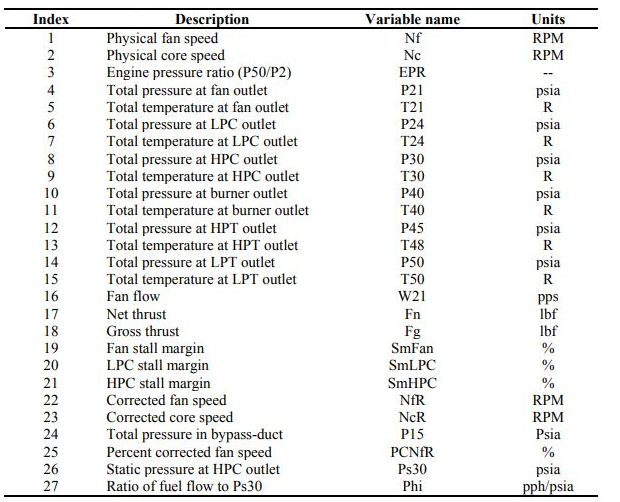
\includegraphics[scale=0.5]{animate/sensores.png}
        \caption{Sensores o variables de salida de software C-MAPSS. \cite{turbofan_nasa}.}
        \label{fig:my_label}
    \end{figure}
\end{frame}

\begin{frame}{Anexos B1}
Ecuaciones LSTM \cite{LSTM},
    \begin{enumerate}
    \begin{equation}
        i_{t}^{j}= \sigma (W_{i}\cdot{x_{t}} + U{i}\cdot{h_{t-1}} + V_{i}\cdot{c_{t-1}}  + b_{i})^{j}
    \end{equation}
    \begin{equation}
        f_{t}^{j}= \sigma (W_{f}\cdot{x_{t}} + U{f}\cdot{h_{t-1}} + V_{f}\cdot{c_{t-1}}  + b_{f})^{j}
    \end{equation}
    \begin{equation}
        \Bar{c}_{t}^{j}= \tanh (W_{c}\cdot{x_{t}} + U{c}\cdot{h_{t-1}} + b_{c})^{j} 
    \end{equation}
    \begin{equation}
         {c}_{t}^{j}= f_{t}^{j}\cdot{c_{t}^{j}} + i_{t}^{j}\cdot{\Bar{c}_{t}^{j}}
    \end{equation} 
    \begin{equation}
          o_{t}^{j}= \sigma (W_{o}\cdot{x_{t}} + U{o}\cdot{h_{t-1}} + V_{o}\cdot{c_{t-1}}  + b_{o})^{j}
    \end{equation}
    \begin{equation}
        {h}_{t}^{j}= o_{t}^{j} \cdot \tanh({c}_{t}^{j})
    \end{equation}
    
\end{enumerate}

    
\end{frame}

\begin{frame}{Anexos B2}
Ecuaciones ConvLSTM \cite{convlstm},
\begin{enumerate}
    \begin{equation}
        i_{t}^{j}= \sigma (W_{i}*{X_{t}} + U{i}*{H_{t-1}} + V_{i}\circ{C_{t-1}}  + b_{i})^{j}
    \end{equation}
    \begin{equation}
        f_{t}^{j}= \sigma (W_{f}*{X_{t}} + U{f}*{H_{t-1}} + V_{f}\circ{C_{t-1}}  + b_{f})^{j}
    \end{equation}
    \begin{equation}
        \Bar{C}_{t}^{j}= \tanh (W_{c}*{x_{t}} + U{c}*{h_{t-1}} + b_{C})^{j} 
    \end{equation}
    \begin{equation}
         {C}_{t}^{j}= f_{t}^{j}\circ{C_{t}^{j}} + i_{t}^{j}\circ{\Bar{C}_{t}^{j}}
    \end{equation} 
    \begin{equation}
          o_{t}^{j}= \sigma (W_{o}*{X_{t}} + U{o}*{H_{t-1}} + V_{o}\circ{C_{t-1}}  + b_{o})^{j}
    \end{equation}
    \begin{equation}
        {H}_{t}^{j}= o_{t}^{j} \cdot \tanh ({C}_{t}^{j})
    \end{equation}
    
\end{enumerate}
\end{frame}

\begin{frame}{Anexos B3}
Ecuaciones JANET \cite{janet},
\begin{enumerate}
    \begin{equation}
        f_{t}^{j}= \sigma (W_{f}*{x_{t}} + U_{f}*{h_{t-1}} + b_{f})^{j}
    \end{equation}

    \begin{equation}
         {c}_{t}^{j}= f_{t}^{j}\odot{c_{t}^{j}} + (1 - f_{t}^{j})\odot{\tanh(W_{c}\cdot{x_{t}} + U_{c}\cdot{h_{t-1}} + b_{c})^{j})}
    \end{equation}
    \begin{equation}
        {h}_{t}^{j}= {c}_{t}^{j}
    \end{equation}
    
\end{enumerate}
\end{frame}

\begin{frame}{Anexos B4}
Ecuaciones ConvJANET

\begin{enumerate}
    \begin{equation}
        f_{t}^{j}= \sigma (W_{f}*{X_{t}} + U_{f}*{H_{t-1}} + b_{f})^{j})
    \end{equation}
    \begin{equation}
         {C}_{t}^{j}= f_{t}^{j}\odot{C_{t}^{j}} + (1 - f_{t}^{j})\odot{\tanh{ (W_{c}*{X_{t}} + U_{c}*{H_{t-1}} + b_{c})^{j} } }
    \end{equation}
    \begin{equation}
        {H}_{t}^{j}= {C}_{t}^{j}
    \end{equation}
    
\end{enumerate}
\end{frame}

\section{Referencias}
\begin{thebibliography}{99}
\begin{frame}{Referencias}


\setbeamertemplate{bibliography item}[online]

\bibitem{engine777}[1] The Seattle Times
    \newblock{Probe of 777 engine’s explosive failure pinpoints its origin, 2015}
\bibitem{bypass_nasa}[2] Turbofan, relación de Bypass 
    \newblock{ Imagen tomada de :\url{https://www.grc.nasa.gov/www/k-12/Missions/Jim/Project2_act.htm}, consultada 06-09-2018)}    
    
%\bibitem{} [2] 

%\bibitem{} [3] 


    
\beamertemplatearticlebibitems
    \bibitem{turbofan_nasa}[3] NASA STI Program
    \newblock{\em \textbf{User’s Guide for the Commercial Modular Aero-Propulsion System Simulation,Version 2}, 2012}    
    
%\beamertemplatearticlebibitems
%    \bibitem{rmse-score}[4] S. Zheng
%    \newblock{\em Imagen tomada de : \textbf{Long Short-Term Memory Network for Remaining
%Useful Life Estimation
%}, 2017}

\beamertemplatearticlebibitems
    \bibitem{estado-arte}[4] Li, Xiang and Ding, Qian and Sun, Jian-Qiao
    \newblock{\em \textbf{Remaining Useful Life Estimation in Prognostics Using Deep Convolution Neural Networks
}, 2017}




    
\end{frame}

\begin{frame}{Referencias}


\beamertemplatearticlebibitems
    \bibitem{NN}[5] F. Rosenblatt
    \newblock{\em \textbf{The Perceptron}, 1958}
    
\beamertemplatearticlebibitems
    \bibitem{CNN}[6] LeCun, Yann and Bernhard E. Boser and John S. Denker and Donnie Henderson and R. E. Howard and Wayne E. Hubbard and Lawrence D. Jackel
    \newblock{\em \textbf{Handwritten Digit Recognition with a Back-Propagation Network}, 1990}    
    
%\beamertemplatearticlebibitems
%    \bibitem{rmse-score}[4] S. Zheng
%    \newblock{\em Imagen tomada de : \textbf{Long Short-Term Memory Network for Remaining
%Useful Life Estimation
%}, 2017}
\beamertemplatearticlebibitems
    \bibitem{LSTM}[7] Hochreiter, Sepp and Schmidhuber, Jürgen
    \newblock{\em \textbf{Backpropagation through time: what it does and how to do it}, 1997}
    
\beamertemplatearticlebibitems
    \bibitem{convlstm}[8] Xingjian Shi and Zhourong Chen and Hao Wang and Dit-Yan Yeung and Wai-Kin Wong and Wang-chun Woo
    \newblock{\em \textbf{Convolutional LSTM Network: A Machine Learning Approach for Precipitation Nowcasting
}, 2015}


    
\end{frame}


\begin{frame}{Referencias}

\beamertemplatearticlebibitems
    \bibitem{janet}[9] Jos van der Westhuizen and
               Joan Lasenby
    \newblock{\em \textbf{The unreasonable effectiveness of the forget gate
}, 2018}

\beamertemplatearticlebibitems
    \bibitem{BPTT}[10] Werbos, Paul
    \newblock{\em \textbf{Backpropagation through time: what it does and how to do it}, 1990}
    
\beamertemplatearticlebibitems
    \bibitem{metricas-rmse}[11] A. Saxena
    \newblock{\em \textbf{damage propagation modeling for aircraft engine run-to-failure simulation}, 2008}    


\beamertemplatearticlebibitems
    \bibitem{E-D1}[12] Srivastava, Nitish and Mansimov, Elman and Salakhutdinov, Ruslan
    \newblock{\em \textbf{Unsupervised Learning of Video Representations Using LSTMs}, 2015}
    
\beamertemplatearticlebibitems
    \bibitem{E-D2}[13] Sutskever, Ilya and Vinyals, Oriol and Le, Quoc V
    \newblock{\em \textbf{Sequence to Sequence Learning with Neural Networks}, 2014}    
\end{frame}

\begin{frame}{Referencias}


\beamertemplatearticlebibitems
    \bibitem{RNN1}[14] Mikolov, Tomas and Karafiát, Martin and Burget, Lukás and Cernocký, Jan and Khudanpur, Sanjeev
    \newblock{\em \textbf{Recurrent neural network based language model}, 2010}
    
\beamertemplatearticlebibitems
    \bibitem{RNN2}[15] Sutskever, Ilya and Vinyals, Oriol and Le, Quoc V
    \newblock{\em \textbf{Generating Sequences With Recurrent Neural Networks}, 2013}    
    
\end{frame}

\end{thebibliography}
\end{document}